\section{Results II: Does the Variance Peak Locate the Transition?}
\label{sec:results-demix}
With the sampler established, we compare the variance-peak estimate with the exact coexistence temperature, first for the single-seed protocol and then with replication.

\subsection{Single-seed and replicated estimates against the exact binodal}
\paragraph{Original single-seed protocol.} The single-seed protocol (E6: $N=100$, one seed per composition, a $20$-point grid on $[1.5,3.0]$) gives the estimates in \cref{tab:repo}. Against the exact binodal they deviate by between $\EsixMinDev$ and $\EsixMaxDev$ (maximum absolute deviation $\EsixMaxAbsDev$), the largest estimate is $\EsixMaxOver$---above $\Tc=\EbHalf$, the highest temperature at which the binodal exists---and the estimates at $f=0.05$ and $f=0.95$, which must coincide by the symmetry of \cref{def:binodal}, differ by $\EsixAsym$. Single-run noise of the size measured below produces features like these. The values lie within $\EsixZMax$ replicate standard deviations of the replicate means at $N=100$ (E5), so a single-seed curve is not evidence for or against any shape of the composition dependence.

\begin{table}[t]
\centering\small
\caption{Estimates of the single-seed protocol (E6; $N=100$, grid step $0.079$) against the exact binodal ($J=1$).}
\label{tab:repo}
\begin{tabular}{@{}cccc@{}}
\toprule
$f$ & $\Tb(f)$ exact & $\hat T^V$ (single seed) & deviation\\
\midrule
0.05 & 2.032 & 1.816 & -0.216 \\
0.10 & 2.188 & 1.974 & -0.214 \\
0.20 & 2.261 & 2.289 & +0.028 \\
0.30 & 2.269 & 2.447 & +0.178 \\
0.40 & 2.269 & 2.447 & +0.178 \\
0.60 & 2.269 & 2.289 & +0.020 \\
0.80 & 2.261 & 2.053 & -0.209 \\
0.95 & 2.032 & 1.579 & -0.453\\
\bottomrule
\end{tabular}
\end{table}

\paragraph{Replicated protocol.} \Cref{fig:demix,tab:demix} report E5 ($\EfiveR$ replicates per cell, all other protocol parameters unchanged). We apply the criteria fixed in \cref{sec:thermo}.
\begin{enumerate}[label=(\roman*),leftmargin=2em]
\item \emph{Single-run noise is large.} The standard deviation of $\hat T^V$ over replicates ranges from $\EfiveSdMin$ to $\EfiveSdMax$ across the $27$ cells, i.e.\ from $2$ to $6$ grid steps.
\item \emph{Central compositions ($0.2\le f\le0.8$).} The bootstrap interval of the replicate-mean peak contains $\Tb(f)$ in $\EfiveCentralIn$ of $\EfiveCentralTot$ cells, but the intervals are wide (widths $\EfiveCIWidthMin$--$\EfiveCIWidthMax$), so the test has little power to distinguish $\Tb(f)$ from values several tenths away. The single-run mean differs from $\Tb$ by more than two standard errors in $\EfiveCenZGtTwo$ of $\EfiveCenTot$ cells (maximum $|z|=\EfiveCenZMax$), with both signs. So the estimator is not unbiased for $\Tb(f)$ in the central range either, but its error there is at most $\EfiveCenBiasMax$, a few grid steps.
\item \emph{Dilute compositions ($f\in\{0.05,0.10,0.95\}$).} Here the estimator is biased \emph{low}: the single-run mean lies between $\EfiveExtBiasMin$ and $\EfiveExtBiasMax$ from $\Tb(f)$, with $|z|\ge\EfiveExtZMin$ in all $9$ cells, and the bootstrap interval contains $\Tb(f)$ in $\EfiveExtremeIn$ of $\EfiveExtremeTot$ cells. At $f=0.05$ the single-run means are $\EfiveMeanAtFiveHundredthXXXII$, $\EfiveMeanAtFiveHundredthLXIV$, $\EfiveMeanAtFiveHundredthC$ for $N=32,64,100$ against $\Tb=\EfiveTbAtFiveHundredth$: over this range of sizes the offset shows no detectable decrease with $N$.
\item \emph{Symmetry.} The estimator should be invariant under $f\leftrightarrow1-f$; \cref{tab:sym} shows differences between $\EfiveSymMin$ and $\EfiveSymMax$ at $N=100$, to be compared with a standard error of about $0.05$ for each entry.
\item \emph{Choice of functional.} The maximiser of the specific heat $\hat T^C$ lies systematically below $\hat T^V$ in the central range (\cref{tab:demix}, last column) and its bootstrap interval contains $\Tb$ in $\EfiveCentralInC$ of $\EfiveCentralTot$ central and $\EfiveExtremeInC$ of $\EfiveExtremeTot$ dilute cells.
\end{enumerate}
The replicated data support the qualitative shape ``roughly flat near $\Tc$ over the central range, lower at dilute compositions'', which is also the shape of $\Tb(f)$. They do not support the claim that the variance peak recovers the binodal quantitatively. At dilute compositions it is statistically distinguishable from $\Tb(f)$. In the central range, its resolution of a few grid steps is larger than the whole composition dependence of $\Tb$, which varies by only $\EbDevTwoTenths$ ($\EbRelTwoTenths\%$) between $f=0.2$ and $f=0.5$ and by $\EbDevThreeTenths$ between $f=0.3$ and $f=0.5$. Differences between central compositions in single-run estimates, such as the peak at $f=0.4$ in the single-seed curve, are noise.

\begin{figure}[t]
\centering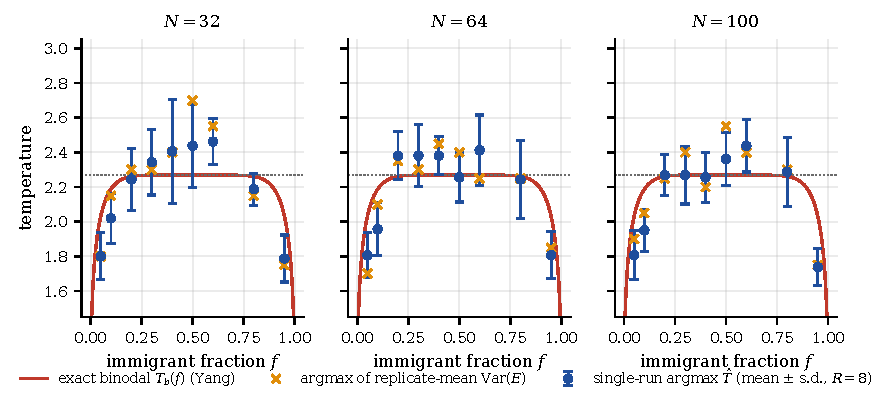
\includegraphics[width=\linewidth]{figures/fig_demixing.pdf}
\caption{\textbf{Variance-peak temperature against the exact coexistence curve} (E5). Blue: mean $\pm$ standard deviation over $\EfiveR$ replicates of the single-run estimator $\hat T^V$ (the original protocol on a grid of step $\EfiveGridStep$); orange crosses: maximiser of the replicate-mean $\Var(E)$; red: exact binodal $\Tb(f)$ (\cref{def:binodal}); dotted: $\Tc$.}
\label{fig:demix}
\end{figure}

\begin{figure}[t]
\centering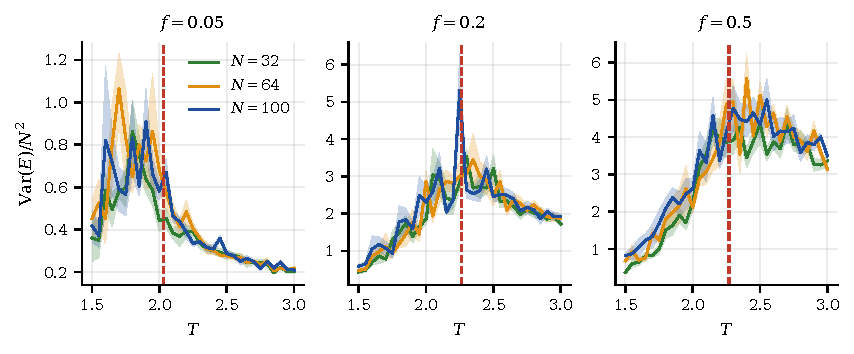
\includegraphics[width=\linewidth]{figures/fig_variance_curves.pdf}
\caption{\textbf{Replicate-mean energy variance per site} for three compositions and three sizes (E5; bands: $\pm1$ s.e.\ over $\EfiveR$ replicates). Dashed red: $\Tb(f)$. The curves are broad and noisy relative to the composition dependence of $\Tb$.}
\label{fig:curves}
\end{figure}

\begin{table}[t]
\centering\small
\caption{Symmetry check of the single-run estimator, $N=100$ (E5): mean of $\hat T^V$ over $\EfiveR$ replicates at $f$ and $1-f$.}
\label{tab:sym}
\begin{tabular}{@{}ccccc@{}}
\toprule
$f$ & $1-f$ & $\langle\hat T^V\rangle_f$ & $\langle\hat T^V\rangle_{1-f}$ & difference\\
\midrule
0.05 & 0.95 & 1.806 & 1.738 & 0.069 \\
0.20 & 0.80 & 2.269 & 2.287 & 0.019 \\
0.40 & 0.60 & 2.256 & 2.438 & 0.181\\
\bottomrule
\end{tabular}
\end{table}
